%!TEX program = xelatex
\documentclass[a4paper,UTF8]{ctexart}
\usepackage[unicode=true,colorlinks,urlcolor=blue,linkcolor=blue,bookmarksnumbered=true]{hyperref}
\usepackage{latexsym,amssymb,amsmath,amsbsy,amsopn,amstext,amsthm,amsxtra,color,multicol,bm,calc,ifpdf}
\usepackage{graphicx}
\usepackage{diagbox}   % 绘制表格斜线
\usepackage{enumerate}
\usepackage{epstopdf}
\usepackage{fancyhdr}
\usepackage{subfigure}
\usepackage{listings}
\usepackage{multirow}
\usepackage{makeidx}
\usepackage{xcolor} 
\usepackage{diagbox}
\usepackage{fontspec}                            % 建立索引宏包
\graphicspath{{figures/}}  % 设置图片搜索路径
\theoremstyle{plain} \newtheorem{theorem}{定理}[section]
\theoremstyle{plain} \newtheorem{definition}{定义}[section]
\theoremstyle{plain} \newtheorem{lemma}{引理}[section]
\theoremstyle{plain} \newtheorem{proposition}{命题}[section]
\theoremstyle{plain} \newtheorem{example}{例}[section]
\theoremstyle{plain} \newtheorem{remark}{注}[section]
\theoremstyle{plain} \newtheorem{corollary}{推论}[section]
\newfontfamily\courier{Courier New}
\lstset{linewidth=1.1\textwidth,
        numbers=left, %设置行号位置 
        basicstyle=\small\courier,
        numberstyle=\tiny\courier, %设置行号大小  
        keywordstyle=\color{blue}\courier, %设置关键字颜色  
        %identifierstyle=\bf,
        commentstyle=\it\color[cmyk]{1,0,1,0}\courier, %设置注释颜色 
        stringstyle=\it\color[RGB]{128,0,0}\courier,
        %framexleftmargin=10mm,
        frame=single, %设置边框格式  
        backgroundcolor=\color[RGB]{245,245,244},
        %escapeinside=``, %逃逸字符(1左面的键),用于显示中文  
        breaklines, %自动折行  
        extendedchars=false, %解决代码跨页时,章节标题,页眉等汉字不显示的问题  
        xleftmargin=2em,xrightmargin=2em, aboveskip=1em, %设置边距  
        tabsize=4, %设置tab空格数  
        showspaces=false %不显示空格  
        basicstyle=\small\courier
       }  
\newenvironment{mysolution}{{\color{blue} 解}: }{{\color{magenta}\qed}}
\newcommand\diff{\,{\mathrm d}} %定义微分d
\newcommand{\p}[3]{\frac{\partial^{#1}#2}{\partial{#3}^{#1}}}  %定义求偏导算子
\newcommand{\ucite}[1]{\textsuperscript{\cite{#1}}}  %参考文献引用:上标用\ucite{ },文中用\cite{ }

\begin{document}
\title{

\includegraphics[width=0.65\textwidth]{onepiece.pdf}\\
\vspace{2em}
\textbf{PageRank 学习笔记}}
\author{\emph{李向阳} \quad {\color{blue} d1142845997@gmail.com}
}
\date{}


\maketitle
\thispagestyle{empty}

\newpage


\tableofcontents

\newpage

\section{引入}
这一次, 我们介绍一下 PageRank 算法.

PageRank 算法曾是谷歌搜索引擎的核心算法. 之前一直听说过谷歌的搜索一开始是凭借算法而名声大震, 但是没有研究过. 这一次就稍微看一下. PageRank 算法是一种网页排序的算法, 刚好契合它的名字, 不过它的命名实际上是源于创始人 Larry Page.

PageRank 算法利用网页链接的关系对网页进行组织, 确定出每个网页的重要级别(PageRank), 简称 PR 值. 当用户进行搜索时, Google 会找出符合搜索要求的网页, 并按照他们的 PR 值排序, 这样用户一般在搜索显示结果的第一页或者前几页就能够找到真正有用的结果.

因此, 关键是计算网页的 PR 值. 对此, PageRank 算法的核心思想有两点:
\begin{enumerate}[(1)]
\item 如果一个网页被很多其他网页链接到的话, 就说明这个网页比较重要, 也就是 PR 值会相对较高;

\item 如果一个 PR 值很高的网页链接到一个其他的网页, 那么被链接到的网页的 PR 值也应该相应的较高.

\end{enumerate}

形象的说, 如果网页 A 链接到网页 B, 则认为“网页 A 给网页 B 了一票”, 而且如果网页 A 的级别越高, 则网页 B 的级别也相应的高(相当于级别高的网页投票的权重也大).

下面的图\ref{example}是一张来自 WikiPedia 的图, 每个球代表一个网页, 球的大小反应了网页的 PR 值的大小. 指向网页 B 和网页 E 的链接很多, 所以 B 和 E 的 PR 值较高, 另外, 虽然很少有网页指向 C, 但是最重要的网页 B 指向了 C, 所以 C 的 PR 值比 E 还要大.
\begin{figure}[!htb]
	\centering
	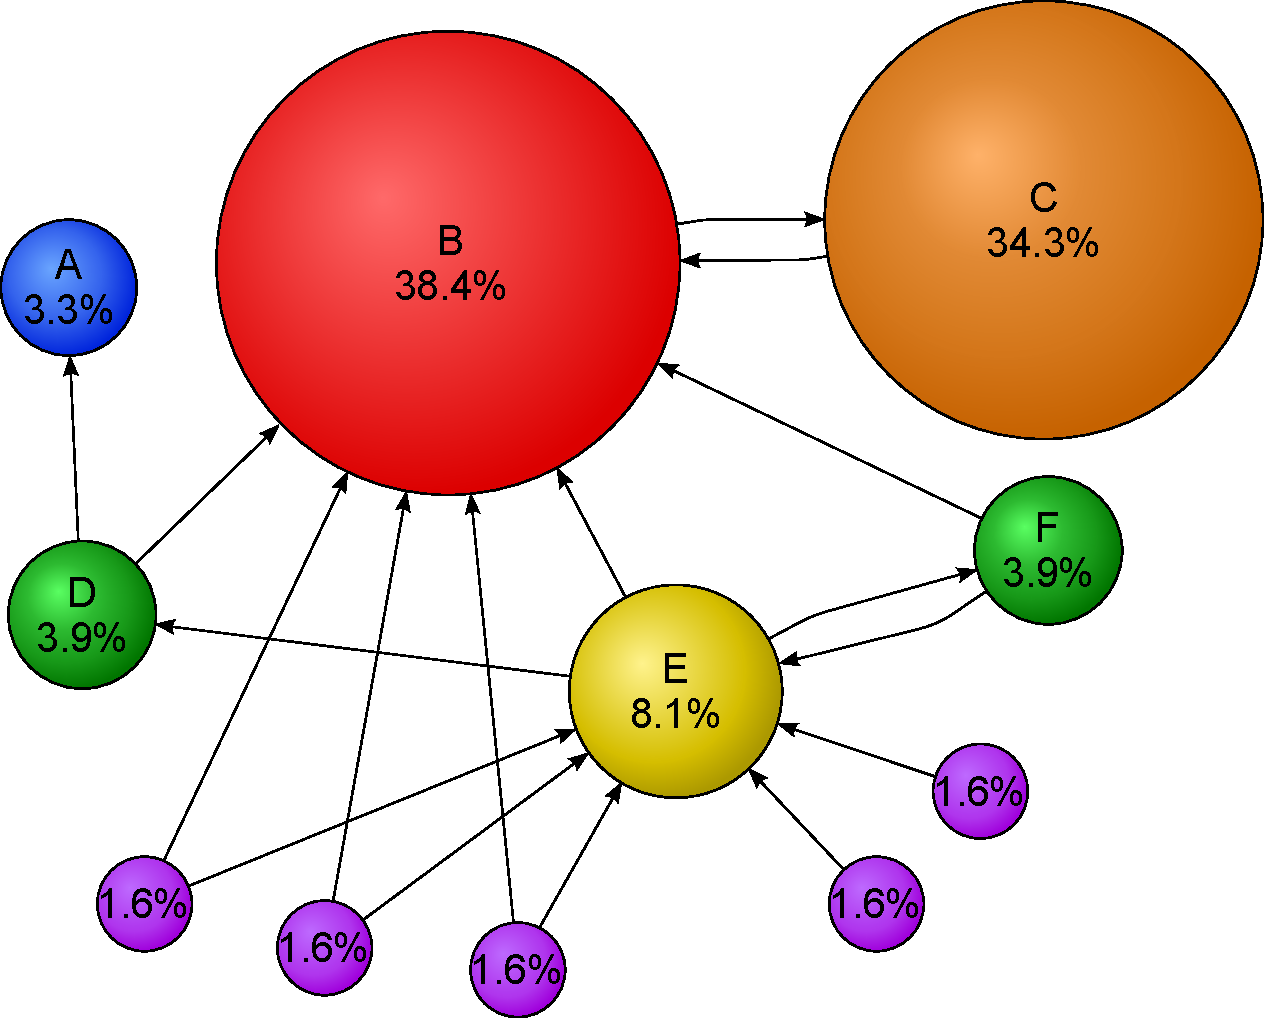
\includegraphics[width = 0.65 \textwidth]{example.pdf}
	\caption{PR 值示意图}
	\label{example}
\end{figure}



有一些网站可以直接给出每个网页(网址)的 PR 值, 比如 \url{http://pr.chinaz.com/}, 下面我们就来介绍 PR 值的计算.


\section{完整模型}
\subsection{模型建立}
假设$n$是 Internet 中所有可访问网页的数目, 注意此数值是非常大的. 我们定义一个$n \times n$的网页链接矩阵, 记为$G = (g)_{ij} \in \mathbb{R}^{n \times n}$, 若从网页$j$有一个链接到网页$i$, 则$g_{ij} = 0$, 否则$g_{ij} = 0$. 矩阵$G$有如下特点:
\begin{enumerate}[(1)]
\item 矩阵$G$是一个大规模稀疏矩阵.

\item 第$i$行非零元素的位置表示了所有链接到网页$i$的网页.

\item 第$j$列非零元素的位置表示了从网页$j$链接出去的所有网页.

\item 矩阵$G$中非零元的数目为整个 Internet 中存在的超链接的数量.

\item 记矩阵$G$第$i$行元素之和为$r_{i} = \sum_{j=1}^{n} g_{ij}$, 它表示第$i$个网页的“入度”.

\item 记矩阵$G$第$j$列元素之和为$c_{j} = \sum_{i=1}^{n} g_{ij}$, 它表示第$j$个网页的“出度”.

\end{enumerate}


要计算 PR 值, 还是需要模型假设的. PageRank 算法便是假设了一个随机上网“冲浪”的过程, 即用户每次看完当前网页后, 有两种选择:
\begin{enumerate}[(1)]
\item 在当前网页中随机选一个超链接进入下一个网页.

\item 随机的新开一个网页.
\end{enumerate}

这在数学上称为马尔科夫过程(Markov Process).真可惜当时在随机过程课上没有讲到这一章. 若这样的随机“冲浪”一直进行下去, 则某个网页被访问到的极限概率就是该网页的 PR 值.

设$p$为选择当前网页上超链接的概率(比如一般取$p = 0.85$), 则$1 - p$为不选当前网页的超链接而随机打开一个新网页的概率. 设当前网页是网页$j$, 我们要计算下一步浏览到达网页$i$的概率(即网页$j$到网页$i$的转移概率), 那么它有两种可能性:
\begin{enumerate}[(1)]
\item 若网页$i$在网页$j$的超链接上, 则其概率为$p \cdot 1 / c_{j} + (1 - p) \cdot 1 / n$;

\item 若网页$i$不在网页$j$的超链接上, 则其概率为$(1 - p) \cdot 1 / n$
\end{enumerate}

由于网页$i$是否在网页$j$的超链接上是由$g_{ij}$决定的, 因此网页$j$到$i$的转移概率为
\begin{equation*}
a_{ij} = g_{ij} \left( p \cdot \frac{1}{c_j} + (1 - p) \cdot \frac{1}{n} \right) + (1 - g_{ij}) \left( (1 - p) \cdot \frac{1}{n} \right) = \frac{p g_{ij}}{c_j} + \frac{1 - p}{n}
\end{equation*}

应当注意的是, 若$c_{j} = 0$, 则也意味着$g_{ij} = 0$, 上式改为$a_{ij} = (1 - p) / n$.

为了表示出概率转移矩阵$A = (a_{ij})_{n \times n}$, 设矩阵$D$表示各个网页出度的倒数(若没有出度, 设为$1$)构成的$n$阶对角阵, $\bm{e}$表示元素全是$1$的$n$维列向量, 则有
\begin{equation*}
A = p G D + \frac{1 - p}{n} \bm{e} \bm{e}^{T}
\end{equation*}

设$x_{i}^{(k)}, i = 1,2,\cdots,n$表示某时刻$k$浏览网页$i$的概率($\sum_{i=1}^{n} x_{i}^{(k)} = 1$), 用向量$\bm{x}^{(k)}$表示$k$时刻浏览各网页的概率分布, 那么下一时刻浏览到网页$i$的概率为$\sum_{j=1}^{n} a_{ij} x_{j}^{(k)}$, 也就是说下一时刻浏览各网页的概率分布为
\begin{equation*}
\bm{x}^{(k+1)} = A \bm{x}^{(k)}
\end{equation*}

当这个过程无限进行下去, 达到极限情况, 可以证明网页访问概率$\bm{x}^{(k)}$会收敛到一个极限值(实际上易知$||A||_{1} = 1$, 因此$\rho (A) \leqslant 1$, 学过数值分析之后这些都很显然了), 这个极限值$\bm{x}$即为各网页的 PR 值, 对上式两边取极限可得$\bm{x}$满足
\begin{equation*}
A \bm{x} = \bm{x}, \sum_{i=1}^{n} x_i = 1
\end{equation*}

也就是说$1$是矩阵$A$的特征值, 而$\bm{x}$即为相应的特征向量, 只要求出这个特征向量即可.


\subsection{用幂法计算 PR 值}
总结以上模型, 给定$n \times n$的网页连接矩阵$G$, 以及选择当前网页超链接的概率$p$, 要计算矩阵$A$的特征值$1$对应的特征向量$\bm{x}$.

实际上, 考虑矩阵$L = I - A$, 容易验证它各列元素之和均为$0$, 因此它是奇异矩阵, 故有$|I - A| = 0$, 因此$1$是矩阵$A$的特征值、主特征值. 更进一步, 可以用圆盘定理考察矩阵$A^{T}$的特征值分布, 下图\ref{circle}显示了第$j$个圆盘$D_{j}(j = 1,2,\cdots,n)$, 显然其圆心$a_{jj} > 0$, 半径$r_j$满足$a_{jj} + r_{j} = 1$, 因此除了$1$这一点, 圆盘上任何一点到圆心的距离(即复数的模)都小于$1$, 这就说明$1$是矩阵$A^{T}$和$A$的唯一主特征值, 因此用幂法求其主特征向量是一个非常不错的选择, 关于幂法理论可回顾数值分析课本. 具体在本模型中, 只要给$\bm{x}$赋予一个初值, 然后重复赋值语句$\bm{x} = A \bm{x}$直到相邻两次计算出的向量的差小于指定精度即可.
\begin{figure}[!htb]
  \centering
  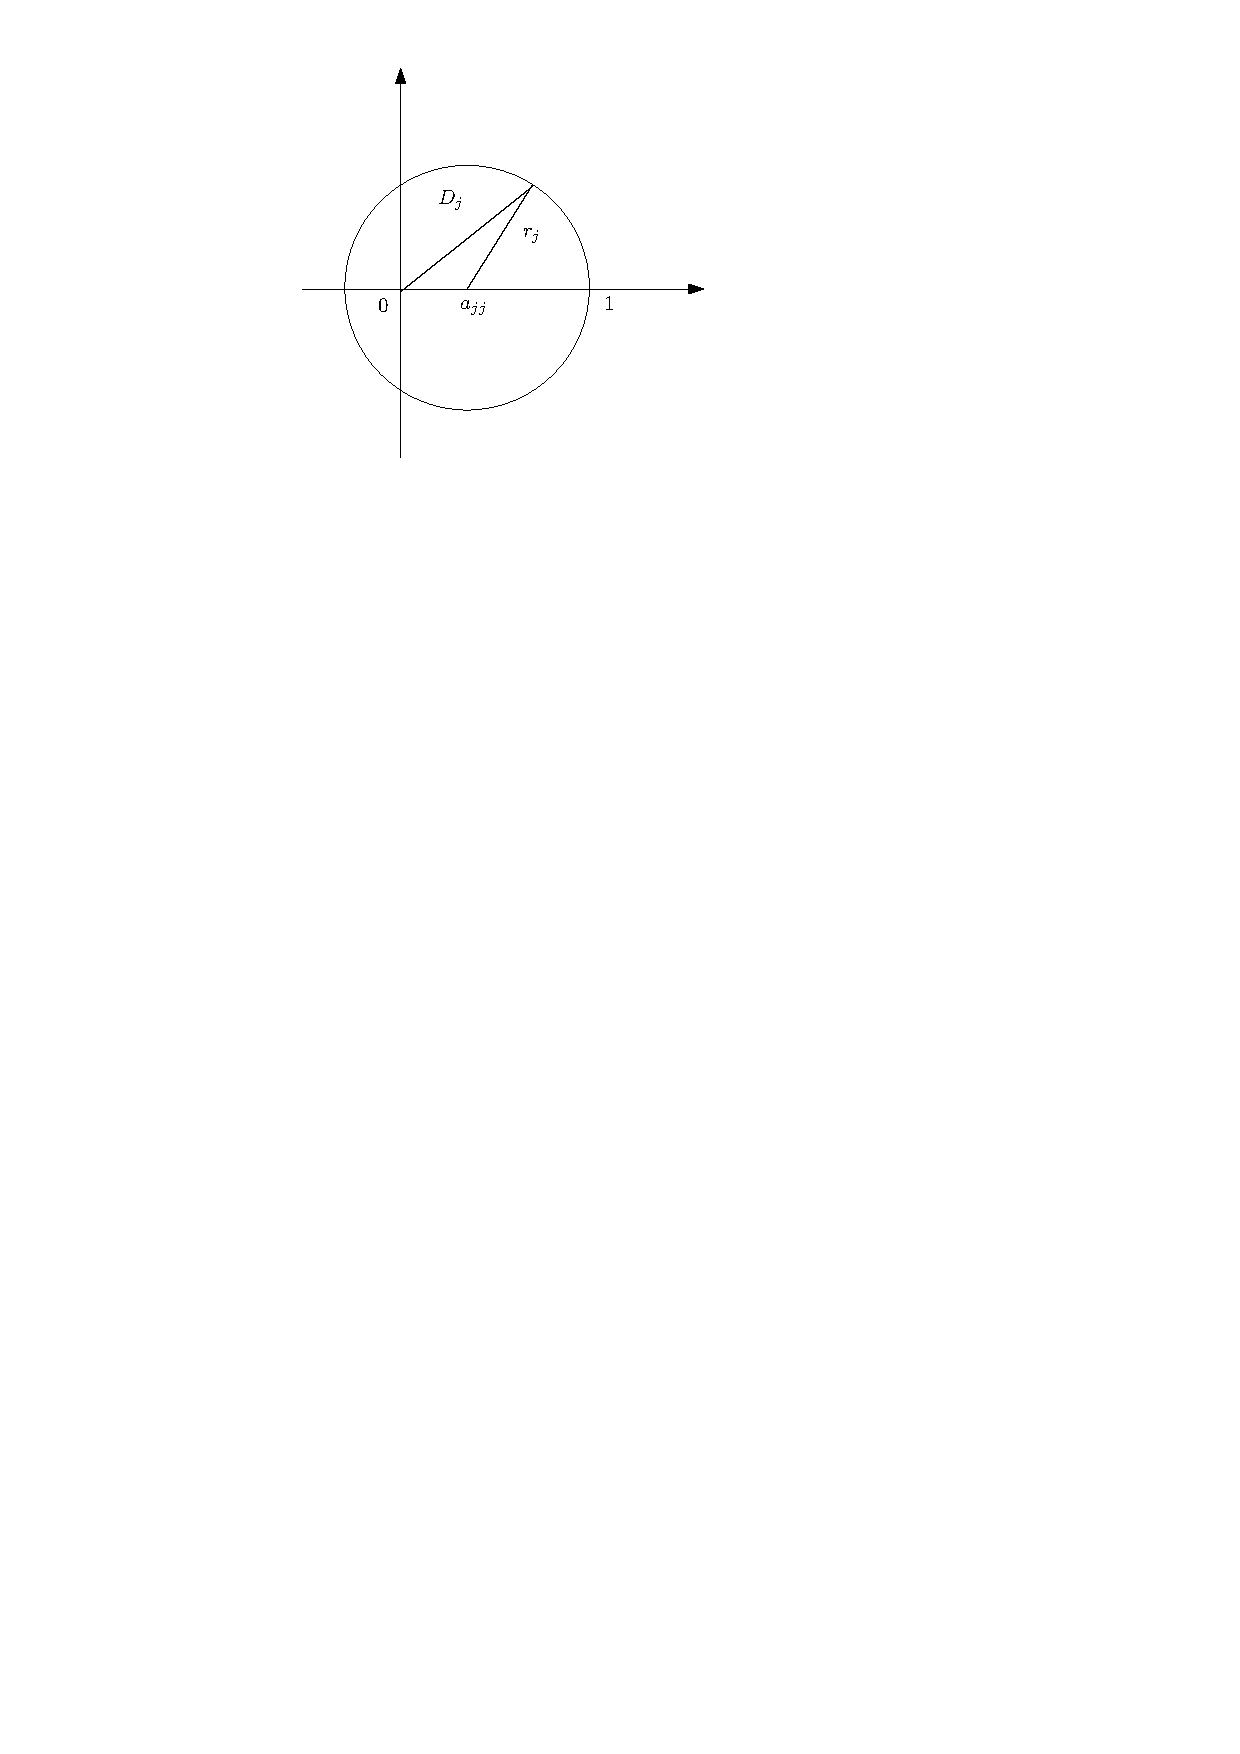
\includegraphics[width=0.65\textwidth]{circle.pdf}
  \caption{矩阵$A^{T}$的第$j$个圆盘}
  \label{circle}
\end{figure}


网页的 PR 值完全由所有网页的超链接结构所决定, 隔一段时间需要重新算一次 PR 值以反映互联网的发展变化, 此时可将上一次的计算结果作为幂法的初始迭代值以提高收敛速度. 由于迭代向量以及矩阵$A$的实际意义, 在使用幂法时并不需要对向量进行规格化, 而且不需要形成矩阵$A$, 通过遍历整个网页的数据库, 根据网页间超链接的关系即可得到$A \bm{x}^{(k)}$的结果.

下面举一个简单例子.
\begin{figure}[!htb]
  \centering
  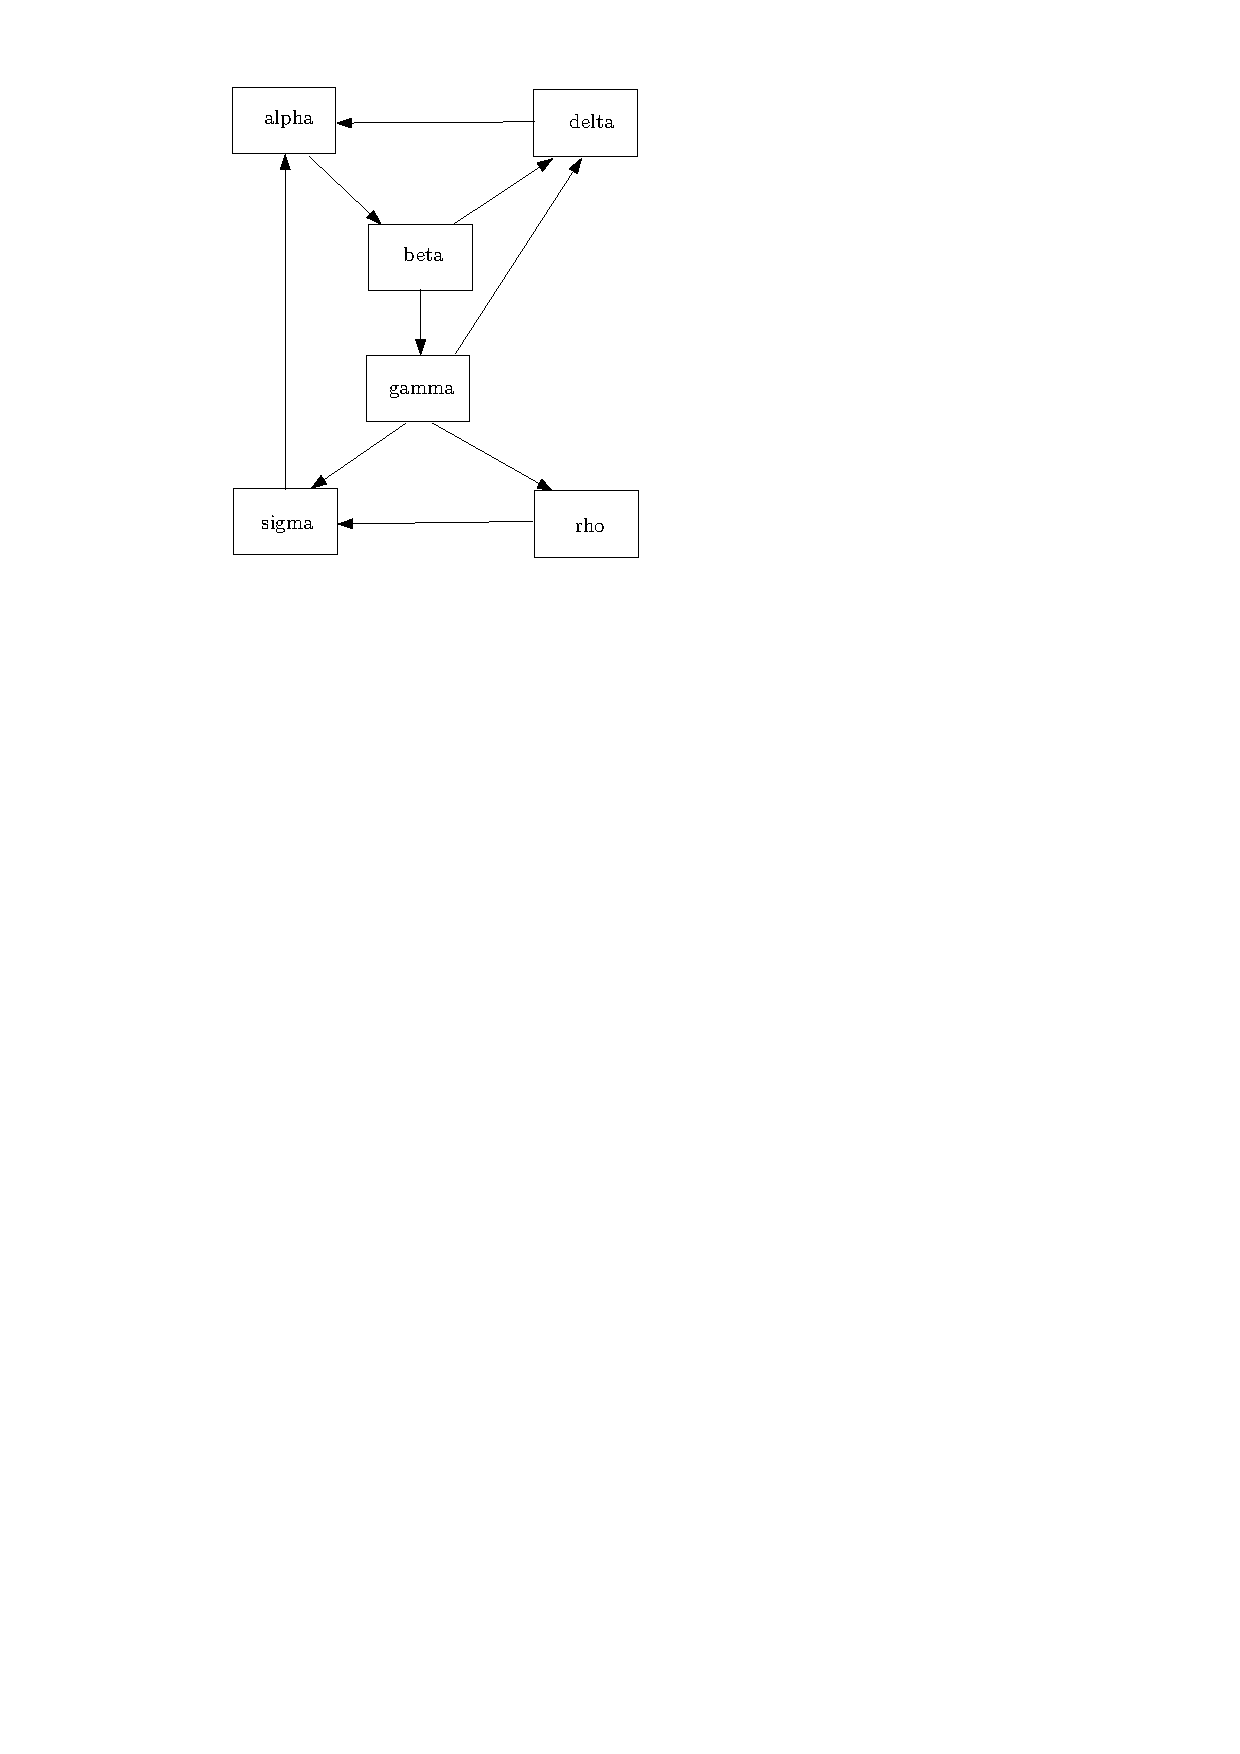
\includegraphics[width=0.75\textwidth]{net.pdf}
  \caption{网页链接示意图}
  \label{net}
\end{figure}

图\ref{net}是一个小规模的网页链接关系图, 这里共有$6$个网页, 即$n = 6$, 其中用 alpha, beta, gamma, delta, rho, sigma 表示网页. 由于连接矩阵$G$是一个稀疏矩阵, 因此我们可以通过指定矩阵非零元素的位置标号$(i,j)$来生成连接矩阵, 由于从 alpha 到 beta 有一个链接, 所以矩阵$G$在位置$(2,1)$就有一个非零元素, 图中的$9$条链接关系可以用
\begin{align*}
i & = [2, 3, 4, 4, 5, 6, 1, 6, 1] \\ 
j & = [1, 2, 2, 3, 3, 3, 4, 5, 6]
\end{align*}

加以表示. 在 Matlab 中, 用如下命令可以生成矩阵$G$
\begin{lstlisting}[language = matlab]
n = 6;
G = sparse(i, j, 1, n, n);
full(G)
\end{lstlisting}

该语句表示矩阵$G$在向量$i$和$j$指定的位置上元素均为$1$, 其余元素默认均为$0$, 用 full 函数可以输出它的完全表示, 如下
$$
G = 
\begin{pmatrix}
0 & 0 & 0 & 1 & 0 & 1 \\ 
1 & 0 & 0 & 0 & 0 & 0 \\ 
0 & 1 & 0 & 0 & 0 & 0 \\ 
0 & 1 & 1 & 0 & 0 & 0 \\ 
0 & 0 & 1 & 0 & 0 & 0 \\ 
0 & 0 & 1 & 0 & 1 & 0 
\end{pmatrix}
$$

再使用如下命令可得到矩阵$A$
\begin{lstlisting}[language = matlab]
c = full(sum(G));
D = spdiag(1./c', 0, n, n);
e = ones(n, 1);
p = 0.85; delta = (1 - p) / n;
A = p * G * D + delta * e * e';
\end{lstlisting}

得到的矩阵$A$为
$$
A = 
\begin{pmatrix}
0.0250 & 0.0250 & 0.0250 & 0.8750 & 0.0250 & 0.8750 \\ 
0.8750 & 0.0250 & 0.0250 & 0.0250 & 0.0250 & 0.0250 \\ 
0.0250 & 0.4500 & 0.0250 & 0.0250 & 0.0250 & 0.0250 \\ 
0.0250 & 0.4500 & 0.3083 & 0.0250 & 0.0250 & 0.0250 \\ 
0.0250 & 0.0250 & 0.3083 & 0.0250 & 0.0250 & 0.0250 \\ 
0.0250 & 0.0250 & 0.3083 & 0.0250 & 0.8750 & 0.0250
\end{pmatrix}
$$

使用幂法可求出其主特征向量, 即 PR 值为
\begin{equation*}
\bm{x} = (0.2675, 0.2524, 0.1323, 0.1697, 0.0625, 0.1156)^{T}
\end{equation*}

用 Matlab 的 bar 命令, 可以将$\bm{x}$的各分量显示如图\ref{bar}所示. 从中可以看出各个网页的级别高低. 虽然链接数目一样, 但网页 alpha 的级别比 delta 和 sigma 都高, 而 beta 的级别第二高, 因为高级别的 alpha 链接到了它上面, 它沾了 alpha 的光.
\begin{figure}[!htb]
  \centering
  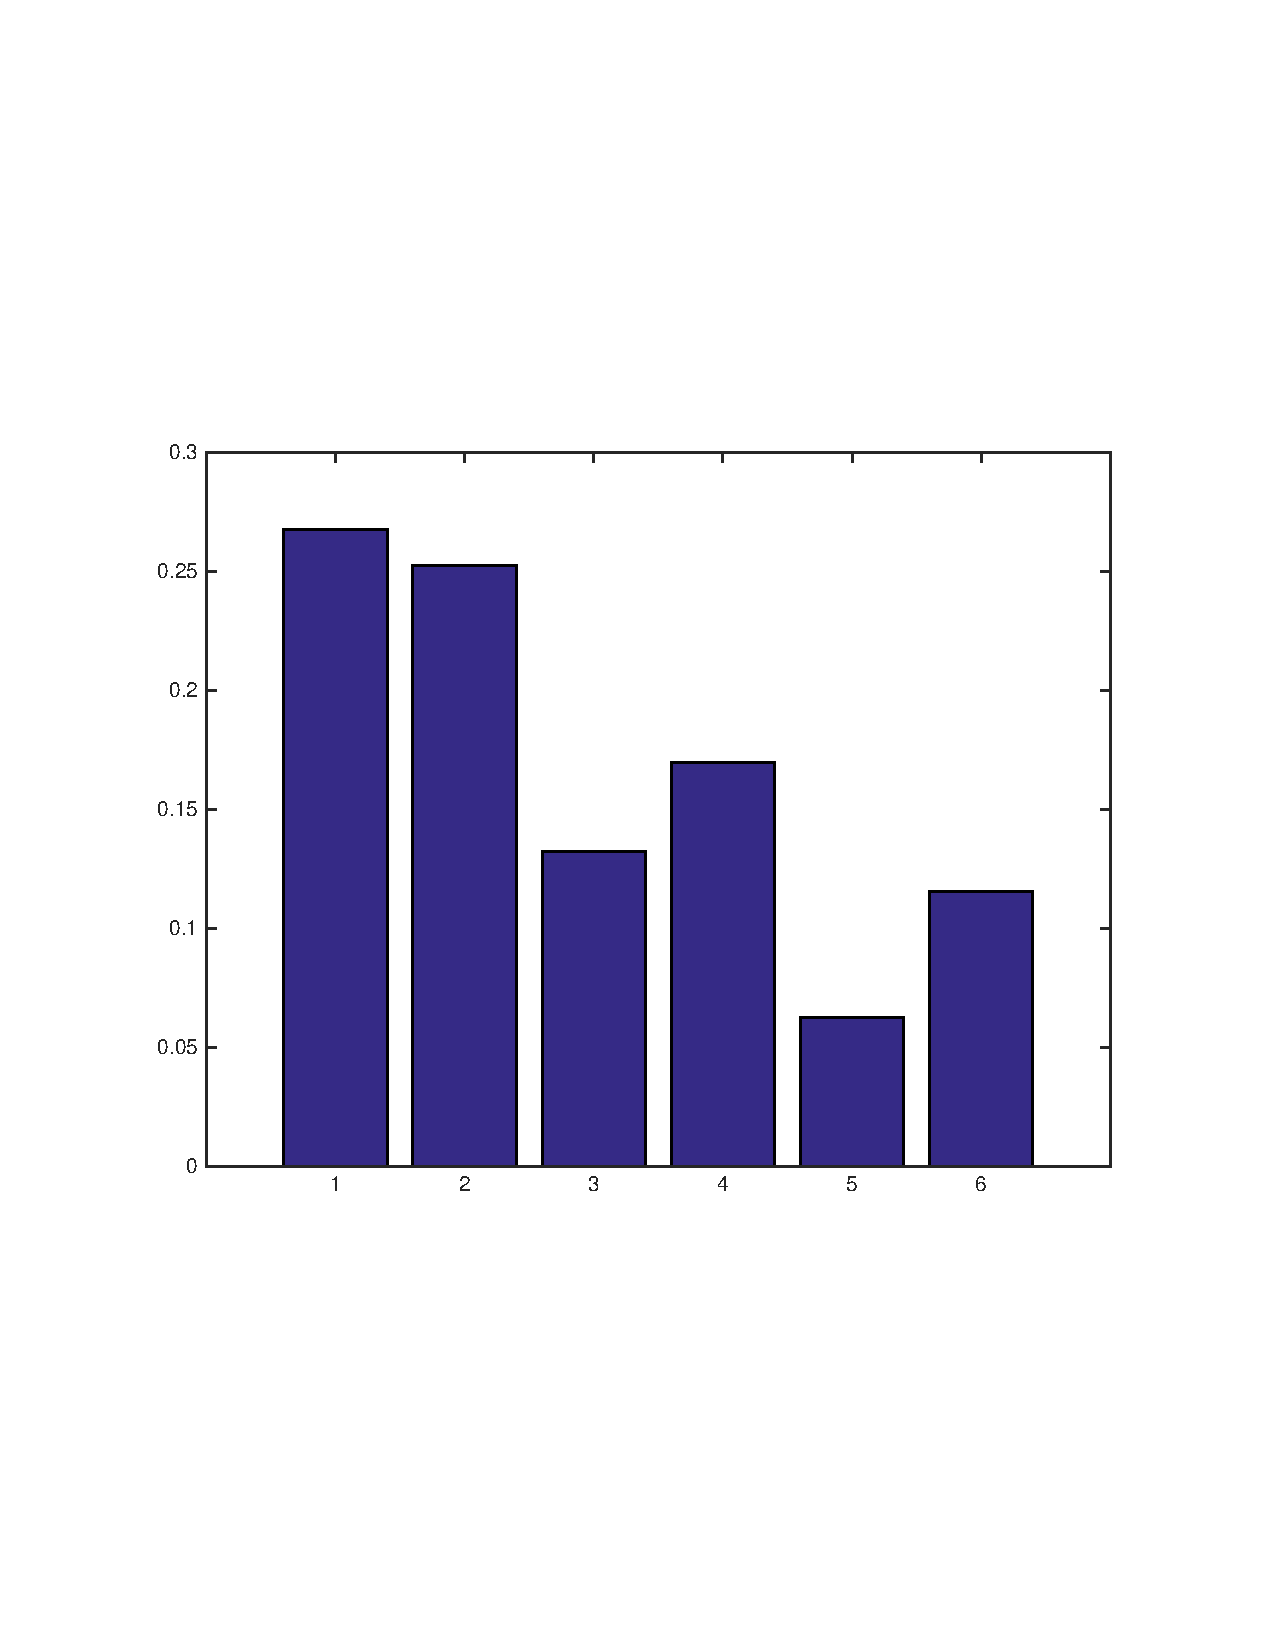
\includegraphics[width=0.75\textwidth]{bar.pdf}
  \caption{PR 值示意图}
  \label{bar}
\end{figure}

除了幂法之外, 还有多种方法计算 PR 值, 比如利用马尔科夫矩阵的特殊结构, 方程
\begin{equation*}
\bm{x} = A \bm{x}
\end{equation*}

可以写成
\begin{equation*}
\bm{x} = (p G D + \delta \bm{e} \bm{e}^{T}) \bm{x}
\end{equation*}

其中为了表示方便, 我们令$\delta = (1 - p) / n$.

注意到$\bm{e}^{T} \bm{x} = 1$, 因此上面的方程变为
\begin{equation*}
(I - p G D) \bm{x} = \delta \bm{e}
\end{equation*}

只要$p$严格小于$1$, 系数矩阵$I - p G D$就是非奇异矩阵, 可根据这个方程解出$\bm{x}$. 此方法保留了矩阵$G$的稀疏性, 但当$p \rightarrow 1$和$\delta \rightarrow 0$时无法使用. 在 Matlab 中, 直接用右除命令即可解方程组
\begin{lstlisting}[language = matlab]
x = (I - p * G * D) \ (delta * e)
\end{lstlisting}


\section{简化模型}
网上很多资料介绍 PageRank 算法时, 是从简化模型开始的, 然后在引入概率参数$p$得到了完整模型. 这里也稍微介绍一下.

在简化模型中, 我们假设上网者每次都是从当前网页的超链接中随机点击一个进去, 而不会随机的新开一个网页, 相当于设定了$p = 1$, 从而概率转移矩阵的元素为
\begin{equation*}
a_{ij} = \frac{g_{ij}}{c_{j}}
\end{equation*}

比如对于图\ref{simple}的网页模型, 其中 A, B, C, D 表示$4$个网页, 那么状态转移矩阵(记为$M$)为
$$
M = 
\begin{pmatrix}
0  &  1 / 2  &  1  &  1 / 3 \\ 
1 / 3  &  0  &  0  &  1 / 3 \\ 
1 / 3  &  0  &  0  &  1 / 3 \\ 
1 / 3  &  1 / 2  &  0  &  0
\end{pmatrix}
$$

\begin{figure}[!htb]
	\centering
	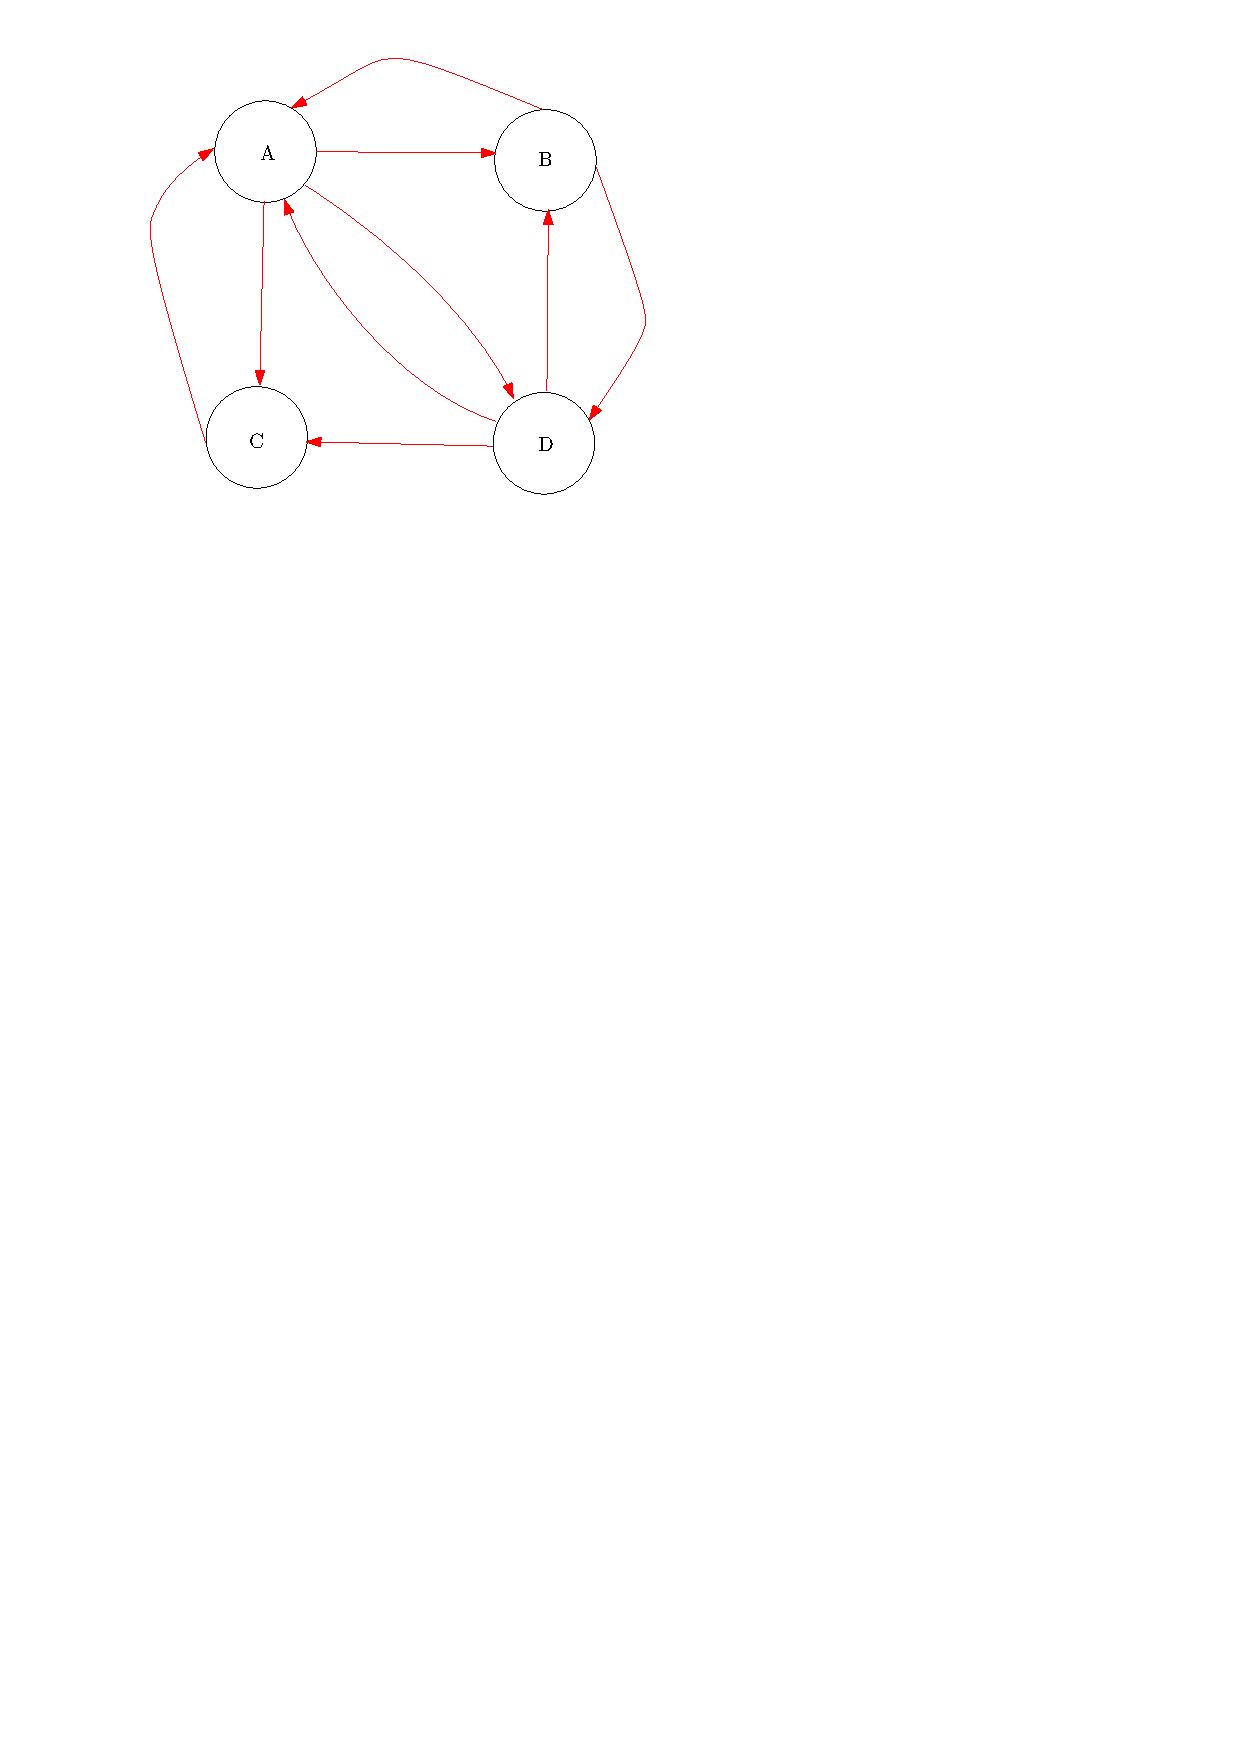
\includegraphics[width = 0.55 \textwidth]{simple.pdf}
	\caption{网页链接示例}
	\label{simple}
\end{figure}

然后迭代计算即可. 实际上, 我们计算下一时刻网页 A 的 PR 值时, 是根据下式计算的
\begin{equation*}
PR(A) = \frac{PR(B)}{2} + \frac{PR(C)}{1} + \frac{PR(D)}{3}
\end{equation*}

其中 B 总共投了$L(B) = 2$票, 其中$1$票给了 A, 即有
\begin{equation*}
PR(A) = \frac{PR(B)}{L(B)} + \frac{PR(C)}{L(C)} + \frac{PR(D)}{L(D)}
\end{equation*}

对于一个页面$u$, 设所有链接到它的页面集合为$B_{u}$, 那么下一轮计算$u$的 PR 值时为
\begin{equation*}
PR(u) = \sum_{v \in B_{u}} \frac{PR(v)}{L(v)}
\end{equation*}


\subsection{简化模型到复杂模型}
上述简化模型会出现问题, 具体可见 \url{http://blog.jobbole.com/71431/} 或者 \url{http://www.changhai.org/articles/technology/misc/google_math.php}, 因此引入了概率参数$p$, 文献上称之为 damping factor(阻尼系数), 即将 PR 值的更新公式改为
\begin{equation*}
PR(A) = \frac{1 - p}{n} + p \left( \frac{PR(B)}{L(B)} + \frac{PR(C)}{L(C)} + \frac{PR(D)}{L(D)} + \cdots \right)
\end{equation*}

这其中$n$为所有网页的个数, 这实际上就是上面完整模型中转移概率$a_{ij}$的计算公式. 

如此一来, 接下来的讨论就和我们上面的完整模型一模一样了, 具体可参见 \url{https://en.wikipedia.org/wiki/PageRank}, 这里就不再多述了.



\section{关于 PageRank 算法的补充}




\section{总结}
\subsection{参考资料}
\begin{enumerate}[(1)]
\item 博客: \url{https://segmentfault.com/a/1190000000711128}, 讲的比较系统而且清楚.

\item 博客: \url{http://www.changhai.org/articles/technology/misc/google_math.php}, 讲述了 PageRank 算法的历史来源, 也有数学上的分析.

\item 博客: \url{http://blog.jobbole.com/71431/}, 从简化的 PageRank 算法讲起, 有问题逐步完善, 同时有 Python 的 Map-Reduce 实现, 讲的不错.

\item 维基: \url{https://en.wikipedia.org/wiki/PageRank}, 从简化模型一直到复杂模型, 讲的很清楚.

\item 博客: \url{http://blog.fens.me/algorithm-pagerank-r/}, 用 R 语言实现了 PageRank 算法, 写的比较清晰.

\end{enumerate}


















\begin{thebibliography}{4}
  \bibitem{1} 李荣华.\emph{偏微分方程数值解法}.高等教育出版社(2010) 
  \bibitem{2} Zhilin Li,Zhonghua Qiao,Tao Tang.\emph{Numerical Solutions of Partial Differential Equations-An Introduction to Finite Difference and Finite Element Methods}.(2011)
  \bibitem{3} 孙志忠.\emph{偏微分方程数值解法}.科学出版社(2011)
  \bibitem{4} 陆金甫 关治.\emph{偏微分方程数值解法}.清华大学出版社(2004)
  
\end{thebibliography}

\newpage

\section*{附录}








\end{document}